\documentclass[12pt]{article}
\usepackage[utf8]{inputenc}
\usepackage{graphicx}
\usepackage{subcaption}
\usepackage{amsmath}
\usepackage{fancyhdr}
\usepackage{geometry}
\usepackage{float}
\usepackage{listings}
\usepackage{xcolor}
\usepackage{array}
\usepackage{caption}
\usepackage{booktabs}
\usepackage[english]{babel}
\usepackage{amssymb}
\usepackage{hyperref}

\lstset{
    basicstyle=\ttfamily\footnotesize,
    backgroundcolor=\color{gray!10},
    keywordstyle=\color{blue},
    commentstyle=\color{green!50!black},
    stringstyle=\color{red},
    numbers=left,
    numberstyle=\tiny\color{gray},
    stepnumber=1,
    numbersep=10pt,
    showstringspaces=false,
    frame=single,
    tabsize=4,
    breaklines=true,
    breakatwhitespace=false,
    language=C
}

\linespread{1.25}
\setlength{\parindent}{0.8cm}
\setlength{\parskip}{0em}
\renewcommand{\headrulewidth}{0pt}
\geometry{a4paper, portrait, margin=1in}
\setlength{\headheight}{14.49998pt}
\graphicspath{{../reports/evidence/L1/}{../reports/evidence/L2/}}

\begin{document}

% ─── TITLE PAGE ───────────────────────────────────────────────────────────────
\begin{titlepage}
  \begin{center}
    \textbf{\large Ministry of Education of Republic of Moldova}\\[0.1cm]
    \textbf{\large Technical University of Moldova}\\[0.1cm]
    \textbf{\large Faculty of Computers, Informatics and Microelectronics}\\[1.2cm]

    \vspace{40mm}

    \textsc{\Large Laboratory Work 1 \& 2:}\\[0.2cm]
    \textsc{\Large The OS as a Resource Manager}\\[0.2cm]
    \textsc{\large Track A (Linux) and Track B (xv6)}\\[0.4cm]

    \vspace{65mm}

    \begin{minipage}[t]{0.4\textwidth}
      \begin{flushleft}\large
        \emph{Author:}\\
        st. gr. FAF-242\\[0.4cm]
        \emph{Verified:}\\
        asist. univ.
      \end{flushleft}
    \end{minipage}
    ~
    \begin{minipage}[t]{0.4\textwidth}
      \begin{flushright}\large
        \emph{}\\
        Tacu Igor\\[0.4cm]
        \emph{}\\
      \end{flushright}
    \end{minipage}\\[2cm]

    \vspace{5mm}
    \large Chi\c{s}in\u{a}u -- 2026

    \vfill
  \end{center}
\end{titlepage}

% ─── TABLE OF CONTENTS ────────────────────────────────────────────────────────
\clearpage
\thispagestyle{empty}
\tableofcontents

\clearpage
\setcounter{page}{2}
\pagestyle{fancy}
\fancyhf{}
\rhead{\thepage}

% ─── OBJECTIVE ─────────────────────────────────────────────────────────────
\section*{OBJECTIVE}
\addcontentsline{toc}{section}{OBJECTIVE}

\hspace{0.8cm} The objective of these two laboratory works is to see, first hand,
how an operating system manages the four resources introduced in the lecture:
files, processes, memory, and devices. Lab 1 (Track A) approaches this from the
outside, observing a real Linux virtual machine through standard commands. Lab 2
(Track B) approaches it from the inside, by building a small teaching operating
system, xv6, from source, using it, reading its kernel/user split, and extending
it with a new program.

% ════════════════════════════════════════════════════════════════════════════
\section*{PART I --- LAB 1: THE OS AS A RESOURCE MANAGER (TRACK A, LINUX)}
\addcontentsline{toc}{section}{PART I --- Lab 1: The OS as a Resource Manager (Track A, Linux)}

\hspace{0.8cm} All work for this part was carried out as \texttt{root} on a
Linux VM (\texttt{ubuntu-4gb-hel1-1}), inside a working folder
\texttt{\textasciitilde/os-lab1}.

\subsection*{1. Files and Directories (File Management)}
\addcontentsline{toc}{subsection}{1. Files and Directories}

\hspace{0.8cm} I started by looking around the filesystem tree with \texttt{pwd},
\texttt{ls}, and \texttt{ls -la /}, then checked my home directory with
\texttt{ls -la \textasciitilde} and peeked into \texttt{/etc}. After that I created
a \texttt{demo} folder and put a test file through the create, copy, rename, and
remove cycle, then checked and changed its permission bits with \texttt{chmod}.

\begin{lstlisting}[language=bash, caption={Commands run for file management}]
pwd
ls -la /
ls -la ~
cd /etc/ && ls | head

mkdir demo && cd demo
echo "Hello Operating System" > note.txt
cp note.txt copy.txt
mv copy.txt renamed.txt
ls -l
rm renamed.txt
ls -l note.txt
chmod 600 note.txt
ls -l note.txt
chmod 644 note.txt
ls -l note.txt
\end{lstlisting}

\begin{figure}[H]
  \centering
  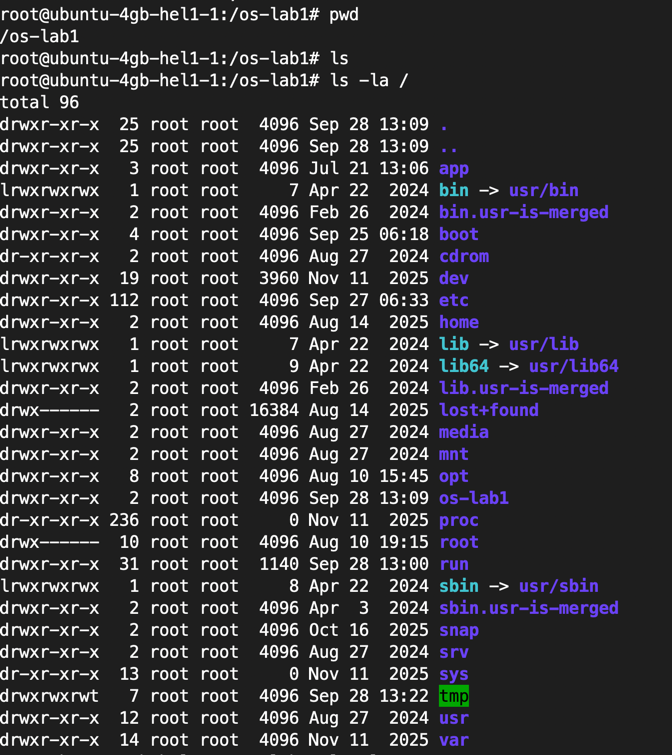
\includegraphics[width=0.85\textwidth]{part1a_pwd_ls_root.png}
  \caption{\texttt{pwd}, \texttt{ls}, and \texttt{ls -la /} on the VM.}
\end{figure}

\begin{figure}[H]
  \centering
  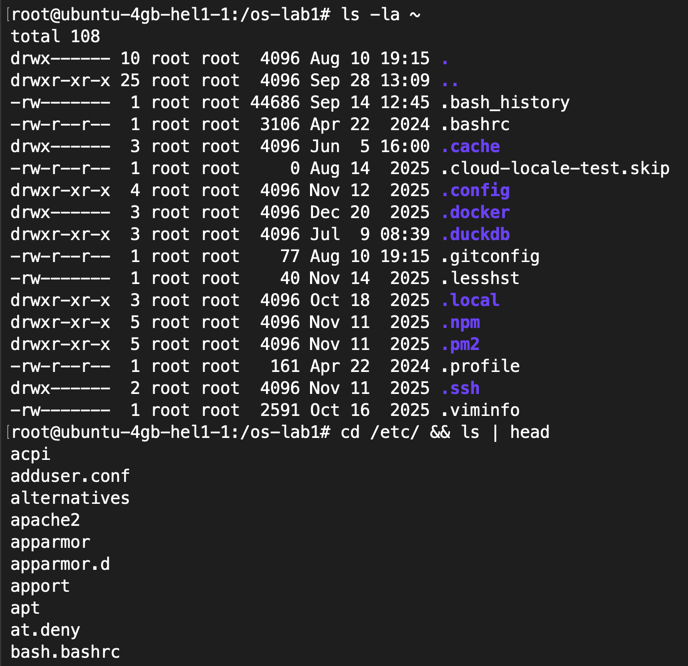
\includegraphics[width=0.85\textwidth]{part1b_ls_home_etc.png}
  \caption{\texttt{ls -la \textasciitilde} and \texttt{cd /etc \&\& ls | head}.}
\end{figure}

\begin{figure}[H]
  \centering
  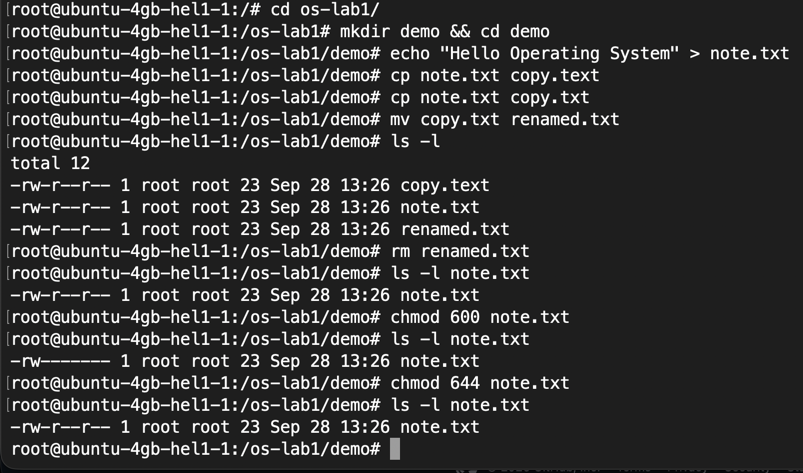
\includegraphics[width=0.85\textwidth]{part1c_mkdir_cp_mv_rm_chmod.png}
  \caption{Create, copy, rename, remove, and \texttt{chmod} cycle in \texttt{demo/}.}
\end{figure}

\noindent\textbf{Observations:}
\begin{itemize}
  \item \textbf{Who owns the files just created, and which group?} \texttt{root:root}.
        Since I was logged in and working as the \texttt{root} user, every file I
        created (\texttt{note.txt}, \texttt{copy.text}, \texttt{renamed.txt}) is
        owned by user \texttt{root} and group \texttt{root}, as shown in the
        \texttt{ls -l} owner/group columns.
  \item \textbf{What do the ten characters at the start of \texttt{ls -l} mean for
        \texttt{note.txt} after \texttt{chmod 600}?} \texttt{-rw-------}: the first
        \texttt{-} marks it as a regular file; the next three (\texttt{rw-}) are
        the owner's permissions (read + write, no execute); the next three
        (\texttt{---}) are the group's permissions (none); the last three
        (\texttt{---}) are everyone else's permissions (none). So only
        \texttt{root} can read or write the file, not even users in the
        \texttt{root} group.
  \item \textbf{Name two directories directly under \texttt{/} and say what they
        hold.} \texttt{/etc} holds system-wide configuration files (e.g.
        \texttt{adduser.conf}, \texttt{apt}, \texttt{bash.bashrc}). \texttt{/root}
        is the home directory of the root user, where my shell's dotfiles
        (\texttt{.bashrc}, \texttt{.ssh}, \texttt{.profile}, etc.) live.
\end{itemize}

\subsection*{2. Processes (Process Management)}
\addcontentsline{toc}{subsection}{2. Processes}

\hspace{0.8cm} I listed the running processes with \texttt{ps aux | head} and
counted them with \texttt{ps aux | wc -l}, then opened \texttt{top} to watch
CPU and memory usage live. Next I put \texttt{sleep 300} in the background, found
it again with \texttt{jobs} and \texttt{ps -ef | grep sleep}, and killed it by
PID. After that I launched another background \texttt{sleep}, looked at
everything the kernel exposes about it under \texttt{/proc/\$PID/}, and read its
\texttt{status} file before killing it too.

\begin{lstlisting}[language=bash, caption={Commands run for process management}]
ps aux | head
ps aux | wc -l
top

sleep 300 &
jobs
ps -ef | grep sleep
kill <PID>

sleep 300 &
PID=$!
ls /proc/$PID
cat /proc/$PID/status | head -20
kill $PID
\end{lstlisting}

\begin{figure}[H]
  \centering
  \begin{subfigure}[t]{0.48\textwidth}
    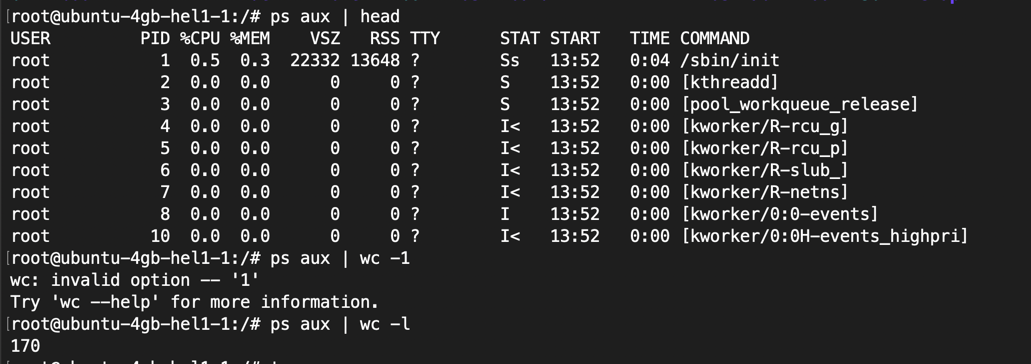
\includegraphics[width=\textwidth]{part2a_ps_aux.png}
    \caption{\texttt{ps aux | head} and process count.}
  \end{subfigure}
  \hfill
  \begin{subfigure}[t]{0.48\textwidth}
    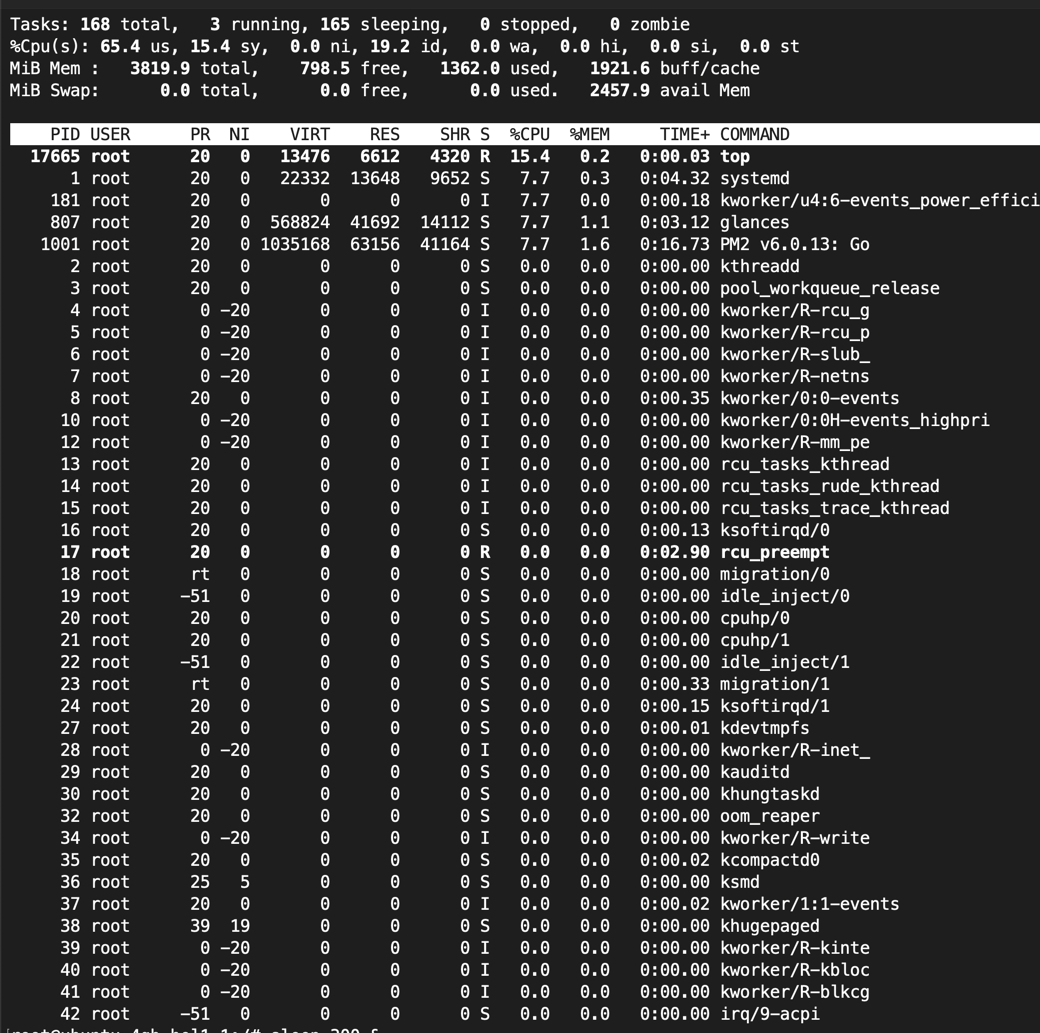
\includegraphics[width=\textwidth]{part2b_top.png}
    \caption{Live view with \texttt{top}.}
  \end{subfigure}
  \caption{Listing and observing processes on the VM.}
\end{figure}

\begin{figure}[H]
  \centering
  \begin{subfigure}[t]{0.48\textwidth}
    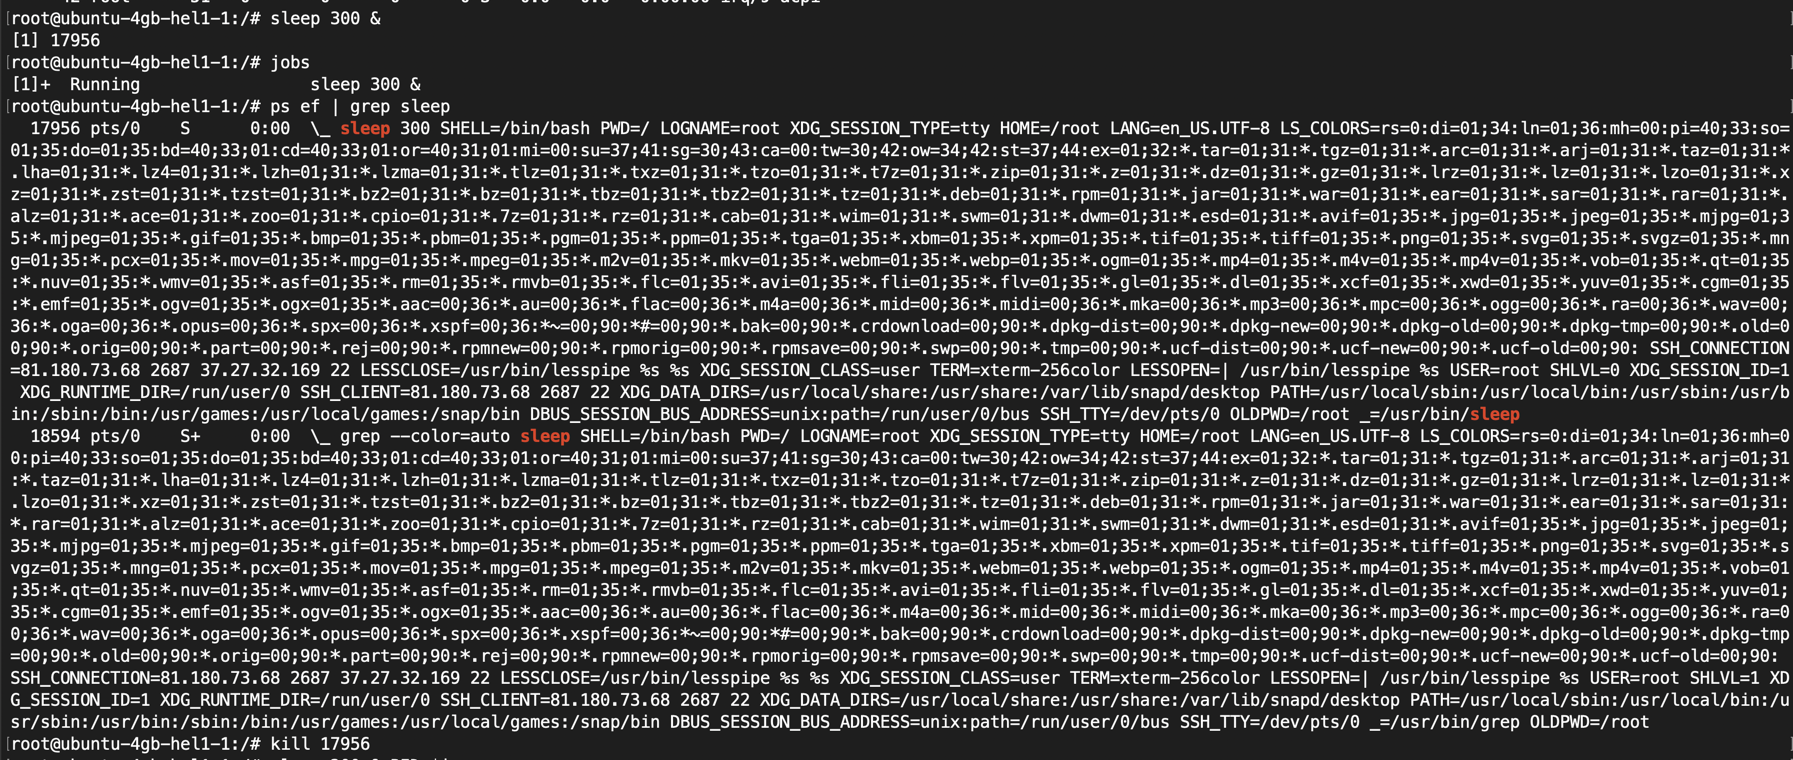
\includegraphics[width=\textwidth]{part2c_sleep_jobs_ps_kill.png}
    \caption{Background \texttt{sleep}, \texttt{jobs}, \texttt{ps -ef}, \texttt{kill}.}
  \end{subfigure}
  \hfill
  \begin{subfigure}[t]{0.48\textwidth}
    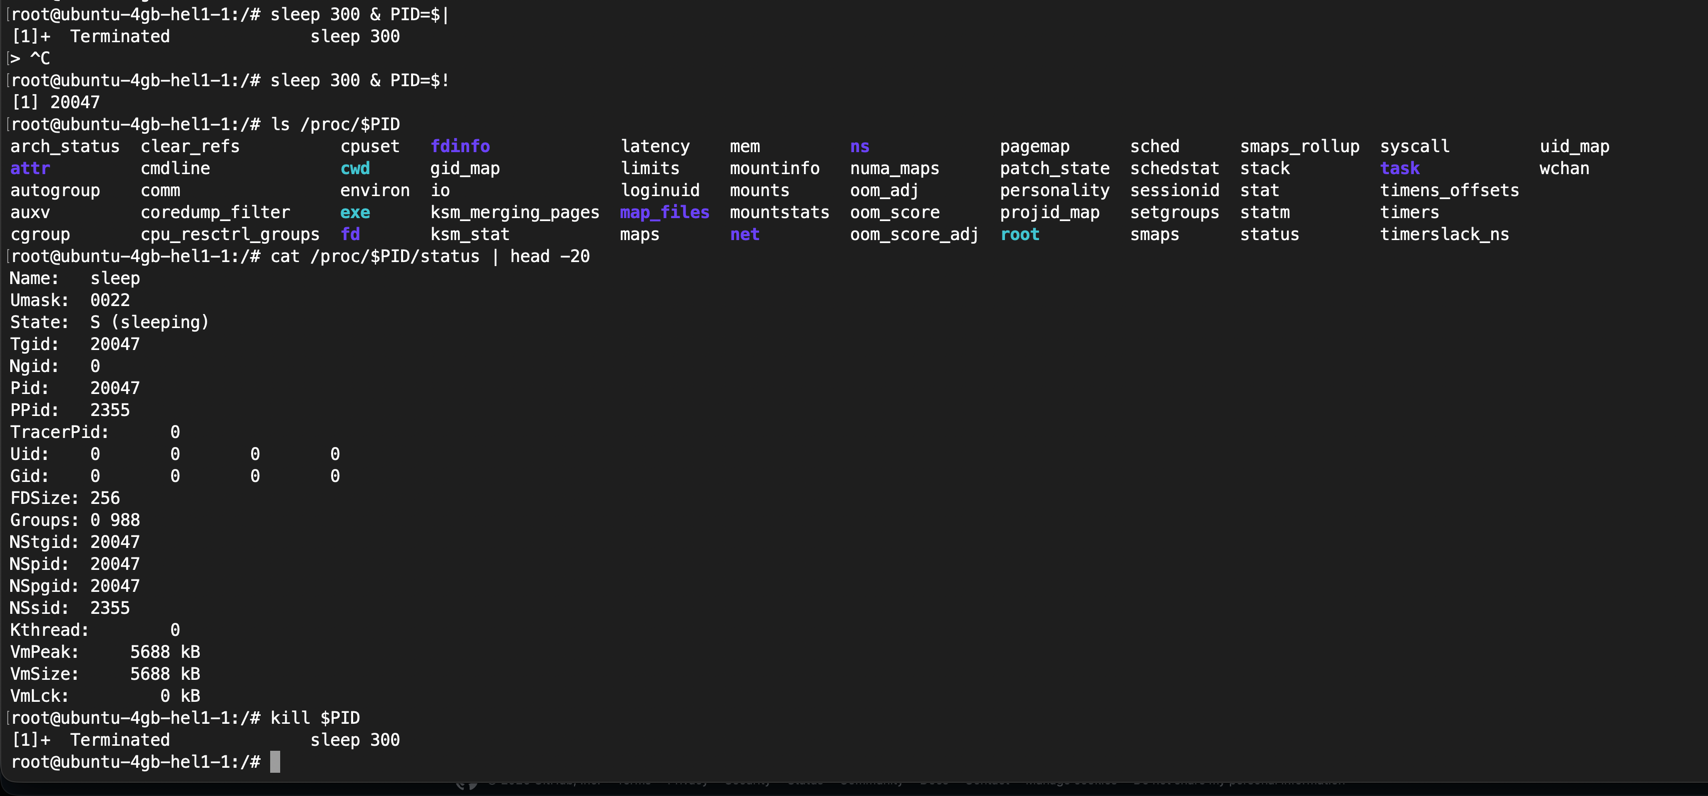
\includegraphics[width=\textwidth]{part2d_proc_pid_status.png}
    \caption{\texttt{/proc/\$PID} exploration and \texttt{status}.}
  \end{subfigure}
  \caption{Background process control and \texttt{/proc} inspection.}
\end{figure}

\noindent\textbf{Observations:}
\begin{itemize}
  \item \textbf{What is the PID of process number 1, and what is it?} PID 1 is
        \texttt{/sbin/init}, the first process the kernel starts at boot, which
        then spawns and supervises (reaps) every other process on the system.
  \item \textbf{Roughly how many processes were running on the idle VM?} About
        170 processes/threads according to \texttt{ps aux | wc -l} (168 tasks
        reported by \texttt{top}, of which 3 running and 165 sleeping).
  \item \textbf{What does the ``State:'' line say for the sleeping process?}
        \texttt{State: S (sleeping)}. The process is blocked waiting on an event
        (here, the \texttt{sleep} timer) and is not consuming CPU while it waits.
\end{itemize}

\subsection*{3. Memory (Memory Management)}
\addcontentsline{toc}{subsection}{3. Memory}

\hspace{0.8cm} I checked the overall RAM/swap totals with \texttt{free -h} and
\texttt{/proc/meminfo}, then started one more background \texttt{sleep 300},
grabbed its PID, and read the \texttt{VmRSS} line from \texttt{/proc/\$PID/status}
to see how much physical RAM a bare \texttt{sleep} process actually uses.

\begin{lstlisting}[language=bash, caption={Commands run for memory management}]
free -h
cat /proc/meminfo | head -6

sleep 300 &
PID=$!
grep VmRSS /proc/$PID/status
kill $PID
\end{lstlisting}

\begin{figure}[H]
  \centering
  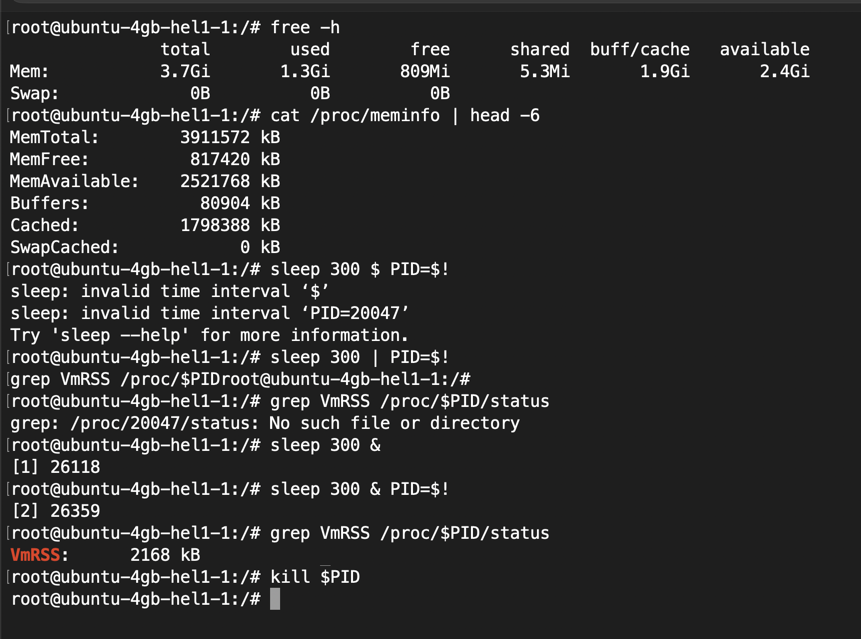
\includegraphics[width=0.85\textwidth]{part3_free_meminfo_vmrss.png}
  \caption{\texttt{free -h}, \texttt{/proc/meminfo}, and \texttt{VmRSS} of a \texttt{sleep} process.}
\end{figure}

\noindent\textbf{Observations:}
\begin{itemize}
  \item \textbf{How much total RAM does the VM have, and how much is free?} The
        VM has 3.7~GiB ($\approx$3,911,572~kB) of total RAM, with 809~MiB
        reported as immediately free and $\sim$2.4~GiB ``available'' once
        reclaimable buffer/cache is counted.
  \item \textbf{What is swap, and how much is configured?} Swap is disk space the
        kernel can use as an overflow for RAM when physical memory runs low,
        swapping out inactive pages. On this VM, swap is \texttt{0B}. None is
        configured, so this instance has no fallback memory beyond physical RAM.
  \item \textbf{How much resident memory (VmRSS) does a bare \texttt{sleep}
        process use?} Only about 2168~kB ($\sim$2.1~MB). That is small, but not
        surprising: \texttt{sleep} is a tiny, statically simple binary that just
        calls \texttt{nanosleep()} and blocks, so it needs almost no working
        memory beyond its loaded code/stack pages.
\end{itemize}

\subsection*{4. Devices and Storage (I/O Management)}
\addcontentsline{toc}{subsection}{4. Devices and Storage}

\hspace{0.8cm} I checked the mounted filesystems and free space with
\texttt{df -h}, looked at the underlying block devices with \texttt{lsblk},
measured my lab folder's size with \texttt{du -sh}, listed device files under
\texttt{/dev}, and sampled the live mount table with \texttt{mount | head}.

\begin{lstlisting}[language=bash, caption={Commands run for devices and storage}]
df -h
lsblk
du -sh ~/os-lab1
ls -l /dev | head
mount | head
\end{lstlisting}

\begin{figure}[H]
  \centering
  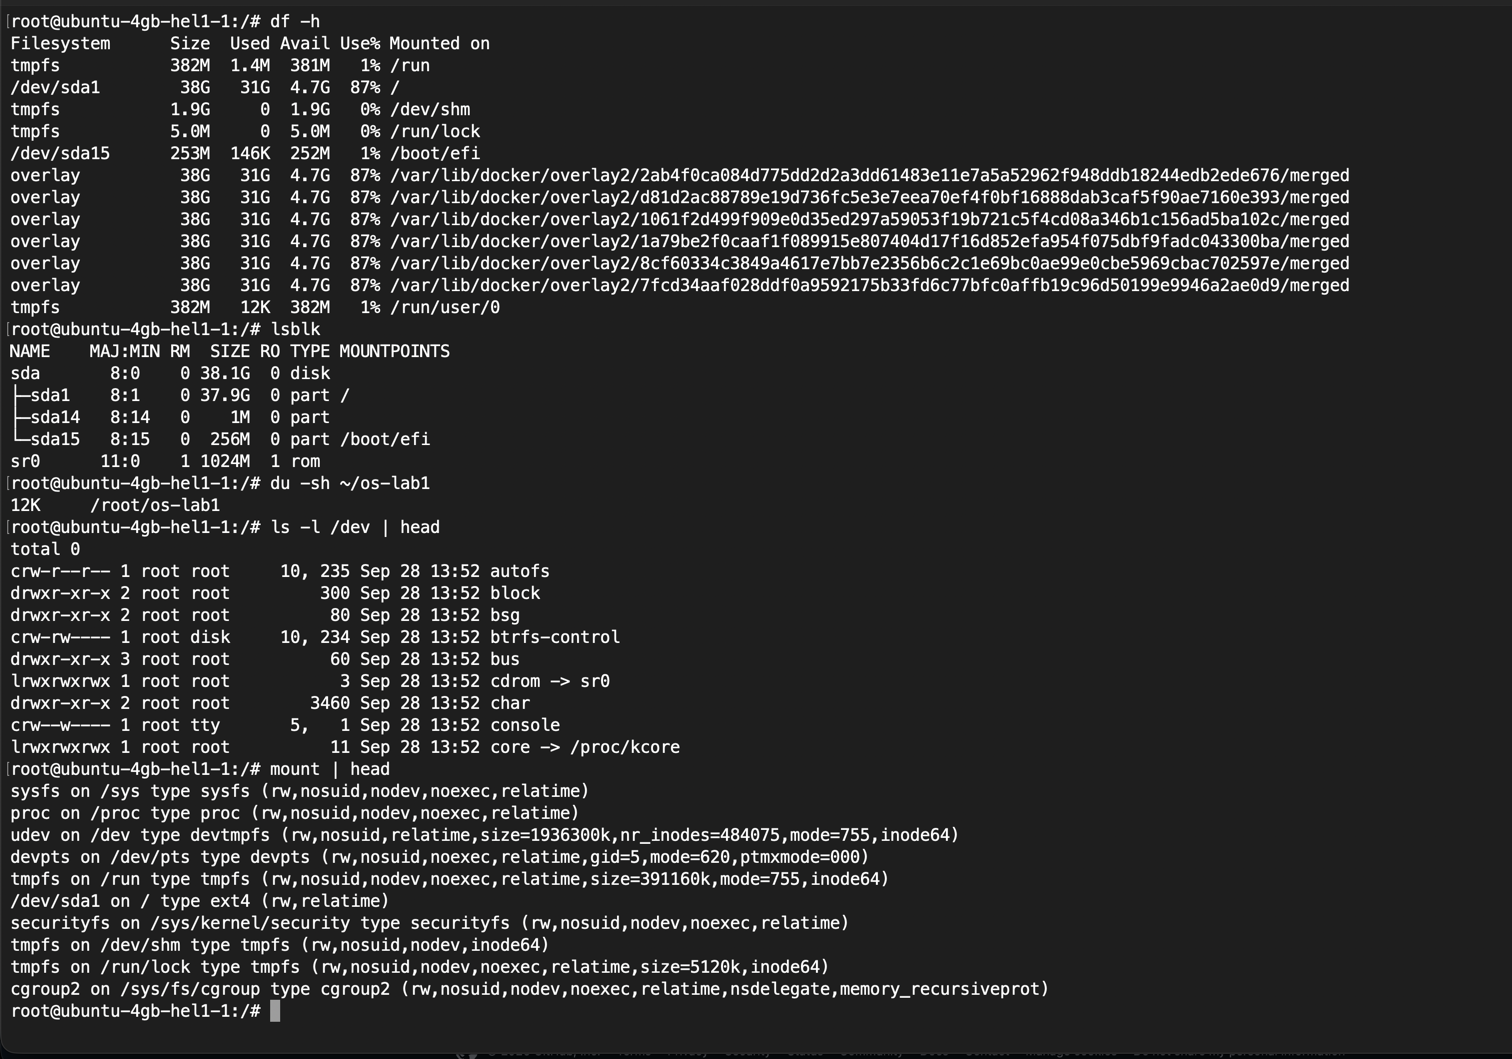
\includegraphics[width=0.85\textwidth]{part4_df_lsblk_dev_mount.png}
  \caption{\texttt{df -h}, \texttt{lsblk}, \texttt{du -sh}, \texttt{/dev}, and \texttt{mount}.}
\end{figure}

\noindent\textbf{Observations:}
\begin{itemize}
  \item \textbf{Which device is the root filesystem ``/'' mounted on?}
        \texttt{/dev/sda1}, an \texttt{ext4} partition (37.9~GiB), as shown by
        both \texttt{df -h} and \texttt{lsblk} and confirmed by \texttt{mount}
        (\texttt{/dev/sda1 on / type ext4}).
  \item \textbf{Give one entry from \texttt{/dev} and what it stands for.}
        \texttt{/dev/console} is a character device (\texttt{crw--w----}, major
        5, minor 1) representing the system console, the device the kernel
        writes boot/system messages to and that early init treats as ``the
        terminal.''
  \item \textbf{What does ``everything is a file'' mean, based on what was
        observed?} It means the kernel exposes hardware and system objects
        (disks like \texttt{/dev/sda1}, the optical drive via
        \texttt{/dev/cdrom} as a symlink to \texttt{sr0}, the console, even
        kernel memory through \texttt{/dev/core} linking to
        \texttt{/proc/kcore}) as ordinary-looking file paths under
        \texttt{/dev}, so the same tools (\texttt{ls}, \texttt{cat},
        permissions, \texttt{read}/\texttt{write}) that work on a text file
        also work on a physical device.
\end{itemize}

\subsection*{Lab 1 --- Synthesis}
\addcontentsline{toc}{subsection}{Lab 1 --- Synthesis}

\hspace{0.8cm} Each part of this lab put one of the OS's four core resources in
front of me. Files: the kernel presents disk storage as a tree of named, owned,
permissioned files, and I could explore and edit that with \texttt{ls -l},
\texttt{chmod}, \texttt{cp}/\texttt{mv}/\texttt{rm}. Processes: every running
program is something the OS created, schedules, and can kill, which
\texttt{ps aux} and \texttt{kill} made visible. Memory: the OS splits physical
RAM between all processes and keeps track of each one's footprint, which
showed up through \texttt{free -h} and the \texttt{VmRSS} line in
\texttt{/proc/<pid>/status}. Devices and I/O: disks, terminals, and other
hardware all sit behind the same file-like interface under \texttt{/dev}, which
\texttt{lsblk} and \texttt{ls -l /dev} made concrete.

% ════════════════════════════════════════════════════════════════════════════
\section*{PART II --- LAB 2: MEET THE OS YOU WILL BUILD (TRACK B, XV6)}
\addcontentsline{toc}{section}{PART II --- Lab 2: Meet the OS You Will Build (Track B, xv6)}

\subsection*{1. Build It and Boot It}
\addcontentsline{toc}{subsection}{1. Build It and Boot It}

\hspace{0.8cm} I cloned xv6 into \texttt{\textasciitilde/xv6-riscv} and ran
\texttt{make qemu}. The first attempt failed immediately:
\texttt{Couldn't find a riscv64 version of GCC/binutils}, and
\texttt{qemu-system-riscv64: not found}. The VM did not have the RISC-V
cross-toolchain or QEMU installed at all, so \texttt{make} fell back to the
system's regular \texttt{gcc} and tried to pass it \texttt{-march=rv64gc},
which is not a valid flag for x86 gcc. I installed the missing pieces
(\texttt{gcc-riscv64-linux-gnu}, \texttt{binutils-riscv64-linux-gnu},
\texttt{qemu-system-misc}), ran \texttt{make clean} to discard the object files
built with the wrong compiler, and re-ran \texttt{make qemu}. This time it
compiled cleanly through the whole kernel and dropped me into the xv6 shell.

\begin{lstlisting}[language=bash, caption={Commands run to build and boot xv6}]
cd ~/xv6-riscv 2>/dev/null || git clone https://github.com/mit-pdos/xv6-riscv ~/xv6-riscv
cd ~/xv6-riscv
ls
make qemu
\end{lstlisting}

\begin{figure}[H]
  \centering
  \begin{subfigure}[t]{0.48\textwidth}
    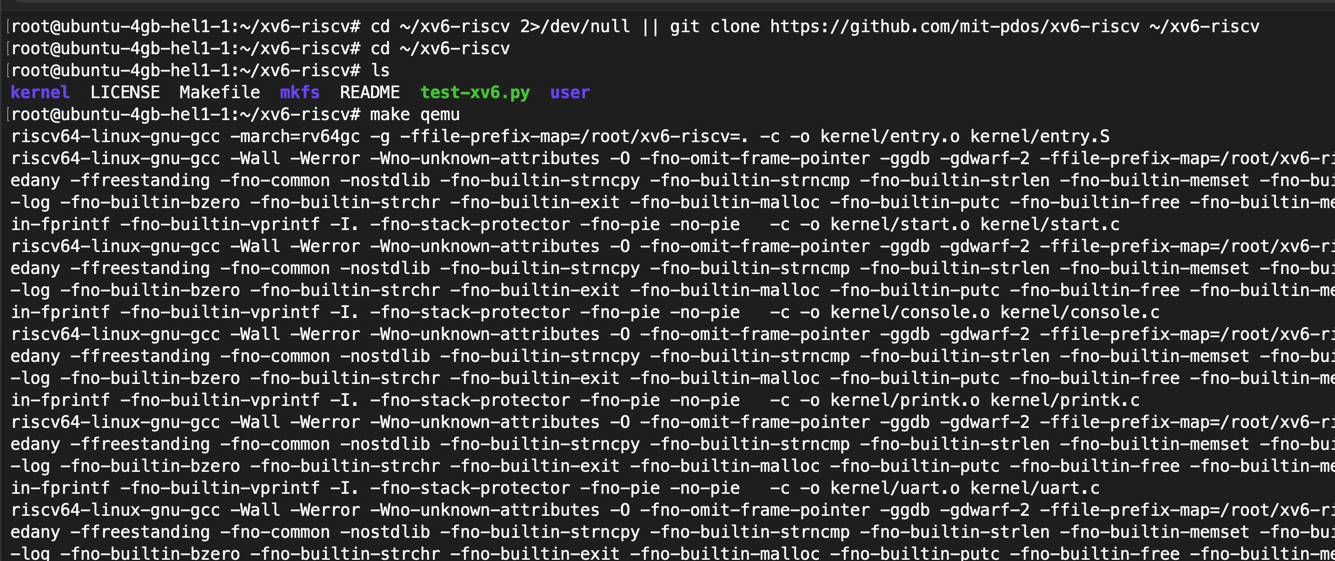
\includegraphics[width=\textwidth]{part1a_clone_and_build_start.png}
    \caption{Cloning the repository and starting the build.}
  \end{subfigure}
  \hfill
  \begin{subfigure}[t]{0.48\textwidth}
    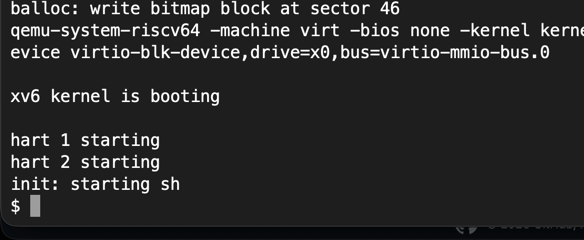
\includegraphics[width=\textwidth]{part1b_boot_success.png}
    \caption{xv6 booted, dropped into the shell.}
  \end{subfigure}
  \caption{Building and booting xv6 in QEMU.}
\end{figure}

\subsection*{2. Use xv6 as the Unix It Is}
\addcontentsline{toc}{subsection}{2. Use xv6 as the Unix It Is}

\hspace{0.8cm} At the \texttt{\$} prompt I ran \texttt{ls} to see what programs
xv6 ships with, \texttt{cat README} to read its own description of itself,
\texttt{echo hello xv6} to check the basics, \texttt{ls | grep c} to confirm
pipes work, and \texttt{wc README} to count lines/words/characters in the
readme.

\begin{lstlisting}[caption={Commands run inside the xv6 shell}]
ls
cat README
echo hello xv6
ls | grep c
wc README
\end{lstlisting}

\begin{figure}[H]
  \centering
  \begin{subfigure}[t]{0.48\textwidth}
    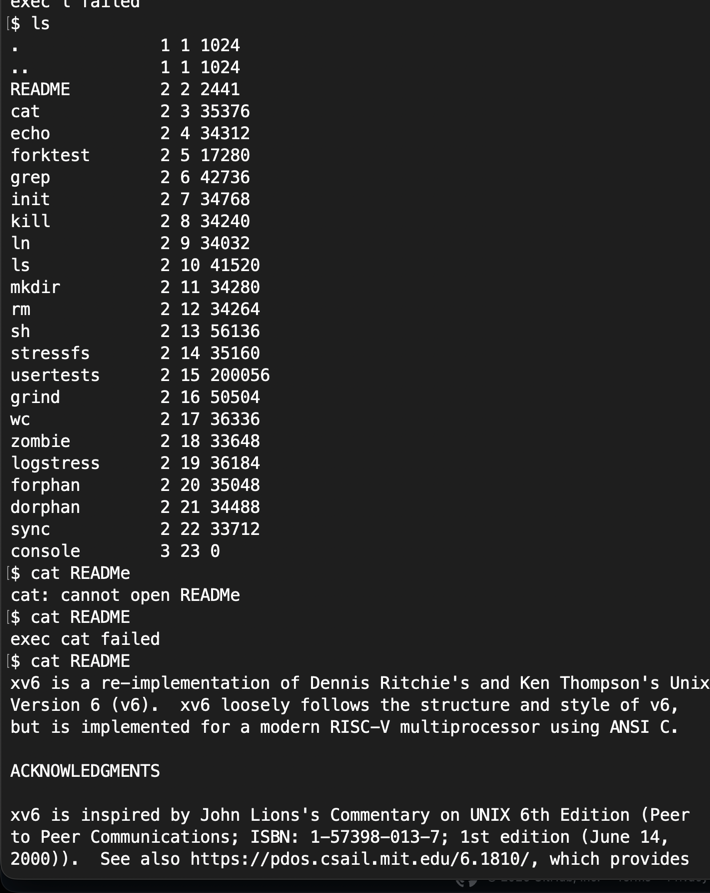
\includegraphics[width=\textwidth]{part2a_ls_and_cat_readme.png}
    \caption{\texttt{ls} and \texttt{cat README}.}
  \end{subfigure}
  \hfill
  \begin{subfigure}[t]{0.48\textwidth}
    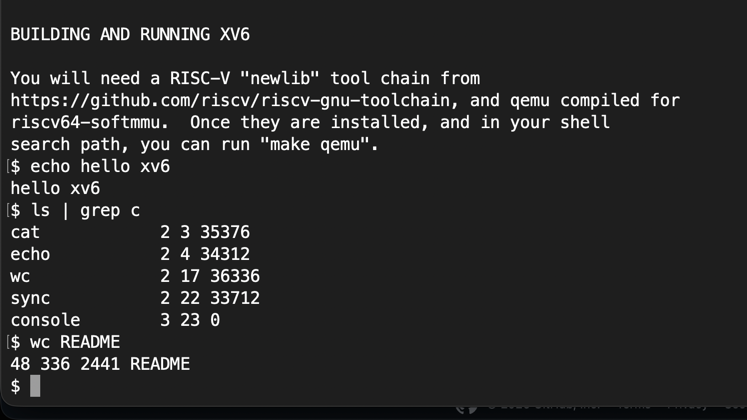
\includegraphics[width=\textwidth]{part2b_echo_pipe_wc.png}
    \caption{\texttt{echo}, a pipe, and \texttt{wc}.}
  \end{subfigure}
  \caption{Using xv6's built-in Unix utilities.}
\end{figure}

\noindent\textbf{Observations:}
\begin{itemize}
  \item \textbf{List three programs xv6 ships with.} From the \texttt{ls}
        output: \texttt{cat}, \texttt{echo}, \texttt{ls} itself, plus others
        like \texttt{grep}, \texttt{wc}, \texttt{sh}, \texttt{init},
        \texttt{kill}, \texttt{mkdir}, \texttt{rm}, \texttt{usertests}.
  \item \textbf{Which two OS features must exist for a pipe to work?}
        Processes and inter-process communication. \texttt{ls | grep c} needs
        two separate processes running at once (the OS's process management),
        and a channel connecting one process's stdout to the other's stdin (the
        OS's pipe/IPC mechanism) so data can flow between them without a file
        on disk.
  \item \textbf{How does the xv6 shell compare to the Linux shell from Lab 1?}
        It is the same idea stripped down to the essentials: xv6's \texttt{sh}
        handles commands, pipes, and redirection just like bash does, just
        without bash's scripting features, job control, or the hundreds of
        built-ins Linux accumulated over the decades.
\end{itemize}

\subsection*{3. Read the Source}
\addcontentsline{toc}{subsection}{3. Read the Source}

\hspace{0.8cm} I exited QEMU (\texttt{Ctrl-A}, then \texttt{X}) and read through
\texttt{user/ls.c} and \texttt{user/cat.c} with \texttt{sed}. Then I opened
\texttt{user/user.h}, which lists every system call a user program is allowed
to make, and grepped \texttt{kernel/sysfile.c} for \texttt{sys\_read}/
\texttt{sys\_write} to see where those calls are actually implemented on the
kernel side.

\begin{lstlisting}[language=bash, caption={Commands run to read the xv6 source}]
sed -n "1,40p" user/ls.c
sed -n "1,30p" user/cat.c
cat user/user.h
grep -n "sys_read\|sys_write" kernel/sysfile.c | head
\end{lstlisting}

\begin{figure}[H]
  \centering
  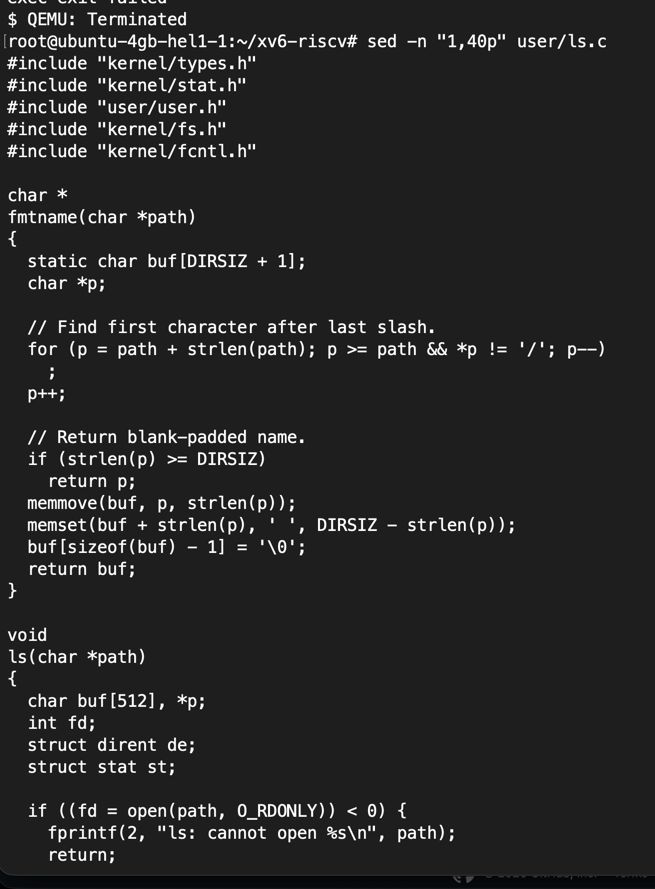
\includegraphics[width=0.85\textwidth]{part3a_ls_c_source.png}
  \caption{\texttt{user/ls.c} source.}
\end{figure}

\begin{figure}[H]
  \centering
  \begin{subfigure}[t]{0.48\textwidth}
    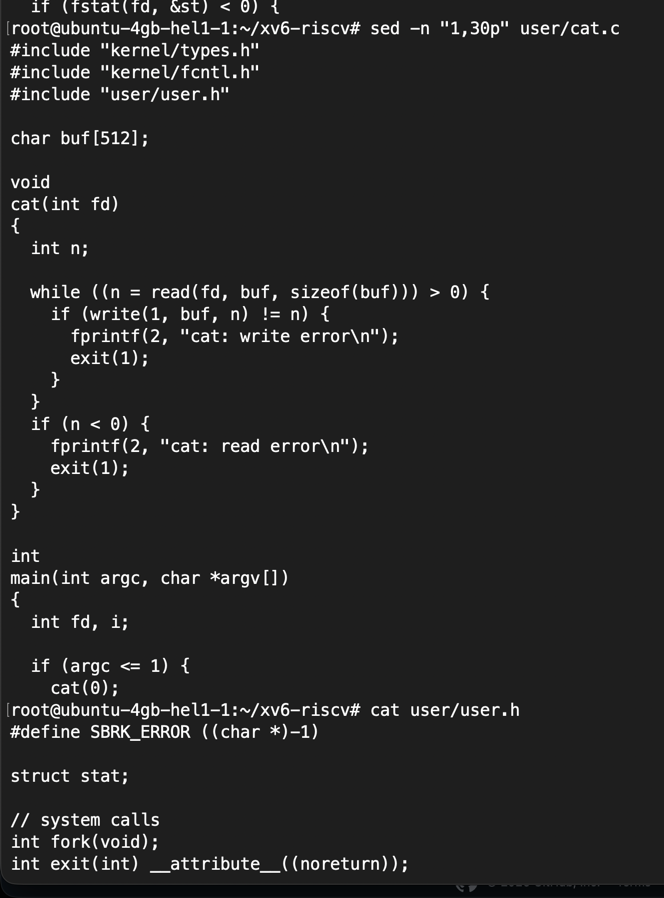
\includegraphics[width=\textwidth]{part3b_cat_c_source_and_userh.png}
    \caption{\texttt{user/cat.c} and the start of \texttt{user.h}.}
  \end{subfigure}
  \hfill
  \begin{subfigure}[t]{0.48\textwidth}
    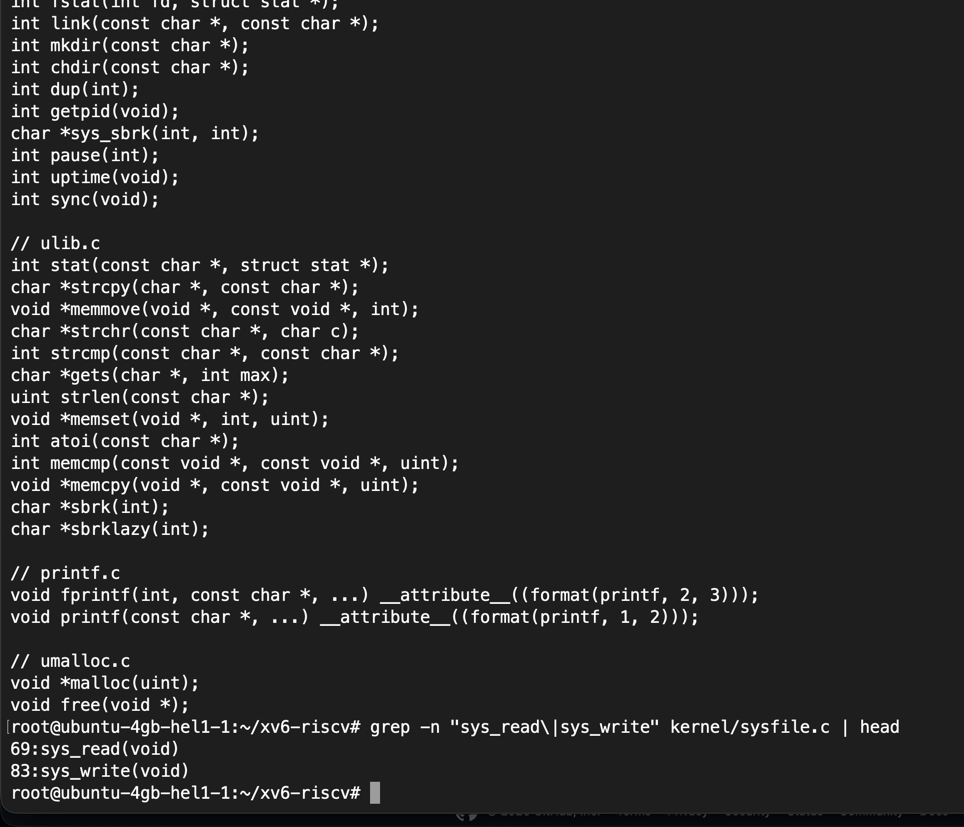
\includegraphics[width=\textwidth]{part3c_userh_and_syscall_grep.png}
    \caption{Rest of \texttt{user.h} and the \texttt{sys\_read}/\texttt{sys\_write} grep.}
  \end{subfigure}
  \caption{Reading the xv6 user-side source and syscall interface.}
\end{figure}

\noindent\textbf{Observations:}
\begin{itemize}
  \item \textbf{Which system calls does \texttt{user/cat.c} use, and what does
        each one ask the kernel to do?} \texttt{read()} and \texttt{write()}.
        \texttt{read(fd, buf, sizeof(buf))} asks the kernel to pull bytes from
        a file descriptor into a buffer, and \texttt{write(1, buf, n)} asks it
        to push bytes from that buffer out to file descriptor 1 (standard
        output). \texttt{cat} itself is just a loop that keeps calling
        \texttt{read} then \texttt{write} until there is nothing left to read.
  \item \textbf{In which kernel file and line is \texttt{sys\_read}
        implemented?} \texttt{kernel/sysfile.c}, line 69 (\texttt{sys\_write}
        sits right below it, at line 83).
  \item \textbf{What is the difference between the code in \texttt{kernel/} and
        the code in \texttt{user/}?} Code in \texttt{kernel/} runs privileged
        and can touch hardware and other processes directly, while code in
        \texttt{user/} runs unprivileged and can only ask the kernel to do
        things on its behalf, through system calls like the ones declared in
        \texttt{user.h}.
\end{itemize}

\subsection*{4. Write My First xv6 Program (\texttt{user/sleep.c})}
\addcontentsline{toc}{subsection}{4. Write My First xv6 Program}

\hspace{0.8cm} I wrote \texttt{user/sleep.c} following the classic xv6 pattern:
check \texttt{argc}, print a usage message and \texttt{exit(1)} if it is wrong,
otherwise call the sleep syscall and \texttt{exit(0)}. My first draft called
\texttt{sleep(atoi(argv[1]))}, the way the lab sheet shows it.

\hspace{0.8cm} Adding it to the build was not quite as smooth as expected.
First I added \texttt{\$U/\_sleep\textbackslash} to the \texttt{UPROGS} list in
the Makefile, but on the first rebuild the binary still was not there and
running \texttt{sleep 10} inside xv6 gave \texttt{exec sleep failed}. The
Makefile edit had not actually landed, so I redid it more carefully and
confirmed with \texttt{grep -A 30 "UPROGS=" Makefile} that
\texttt{\$U/\_sleep\textbackslash} was really in the list this time.

\hspace{0.8cm} That fixed the ``not found'' problem, but then the build itself
broke: \texttt{gcc} reported \texttt{implicit declaration of function
`sleep'}. Checking \texttt{user/user.h} and \texttt{user/usys.pl}, the two
files that together expose a syscall to user programs, showed neither one
mentioned \texttt{sleep} at all. Checking the kernel side
(\texttt{kernel/syscall.h}, \texttt{kernel/syscall.c}) showed why: this
particular xv6 tree does not have a syscall called \texttt{sleep}. It has one
called \texttt{pause} (\texttt{SYS\_pause}, \texttt{sys\_pause}) that does
exactly what the classic \texttt{sleep} syscall does, just under a different
name. So I changed the call in my program from \texttt{sleep(atoi(argv[1]))}
to \texttt{pause(atoi(argv[1]))}, keeping the file named \texttt{sleep.c} and
the usage message unchanged, since the lab only cares about the program's
behavior, not the syscall's internal name. After that, \texttt{make qemu}
built clean and both test cases worked.

\begin{lstlisting}[language=C, caption={Final version of \texttt{user/sleep.c}}, label={lst:sleepc}]
#include "kernel/types.h"
#include "user/user.h"

int
main(int argc, char *argv[])
{
  if(argc != 2){
    fprintf(2, "usage: sleep <ticks>\n");
    exit(1);
  }
  pause(atoi(argv[1])); // system call into the kernel
                         // (this xv6 tree renamed "sleep" to "pause")
  exit(0);
}
\end{lstlisting}

\begin{lstlisting}[language=bash, caption={Commands used to build and test \texttt{sleep}}]
make qemu
sleep 10
sleep
\end{lstlisting}

\begin{figure}[H]
  \centering
  \begin{subfigure}[t]{0.48\textwidth}
    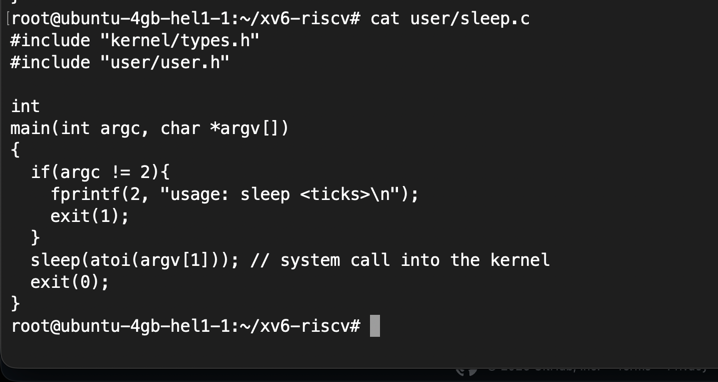
\includegraphics[width=\textwidth]{part4a_first_sleep_c_draft.png}
    \caption{First draft of \texttt{sleep.c}, still calling \texttt{sleep()}.}
  \end{subfigure}
  \hfill
  \begin{subfigure}[t]{0.48\textwidth}
    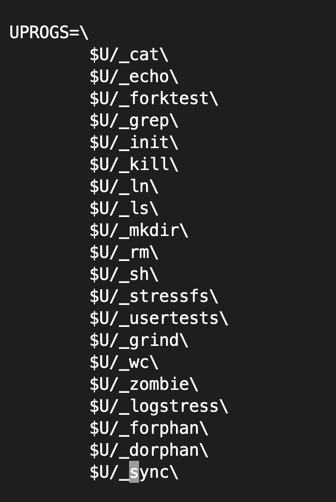
\includegraphics[width=\textwidth]{part4b_makefile_uprogs_before_edit.png}
    \caption{\texttt{UPROGS} list in the Makefile before adding \texttt{sleep}.}
  \end{subfigure}
  \caption{Debugging the build before the fix.}
\end{figure}

\begin{figure}[H]
  \centering
  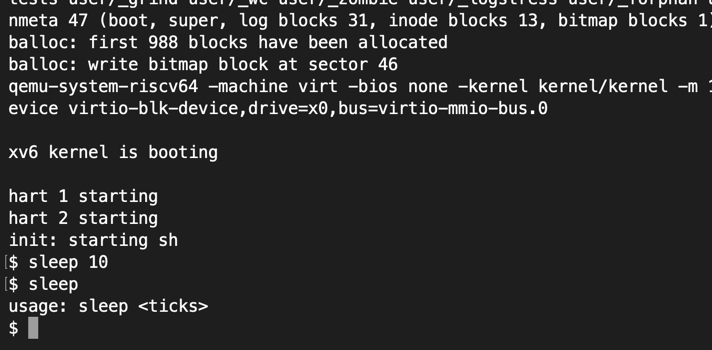
\includegraphics[width=0.85\textwidth]{part4c_sleep_working.png}
  \caption{\texttt{sleep 10} pausing then returning, and \texttt{sleep} printing its usage message.}
\end{figure}

\subsection*{Lab 2 --- Synthesis}
\addcontentsline{toc}{subsection}{Lab 2 --- Synthesis}

\hspace{0.8cm} By the end of this lab I had xv6 built and booted from source,
used it as a small Unix, and read both halves of it: the user programs that
ask for things, and the kernel code that grants them. Writing \texttt{sleep.c}
made that split concrete, since getting it working meant tracing a syscall
from my program, through \texttt{user.h}, into the kernel's syscall table, and
finding out its name had changed along the way. It is a small tree, but I
could hold the whole path in my head while debugging it, which is exactly the
point of using xv6 for this.

% ─── CONCLUSION ────────────────────────────────────────────────────────────
\section*{CONCLUSION}
\addcontentsline{toc}{section}{CONCLUSION}

\hspace{0.8cm} Lab 1 and Lab 2 felt like two ends of the same rope. In Lab 1 I
could only watch Linux from the outside, through \texttt{ps}, \texttt{/proc},
\texttt{ls -l /dev}, and infer what the kernel must be doing behind those
interfaces. In Lab 2 I got to see the other side directly: the actual C code
that implements a syscall, and what happens when a user program's idea of that
syscall does not match the kernel's. The \texttt{pause}/\texttt{sleep}
mismatch in Lab 2 was a good example of something Lab 1 could only hint at:
processes ask the kernel for things by name and number, and if the two sides
disagree on either, nothing works, no matter how correct the surrounding code
looks in isolation.

\pagebreak
\end{document}
